\definecolor{Sail}{rgb}{0.643,0.819,0.976}
En este capítulo se abordarán los diferentes tipos de incertidumbre de medición y se explicará los conceptos teóricos para obtener la incertidumbre expandida. Posteriormente, se revisará la importancia del certificado de calibración y su relación con la trazabilidad de las mediciones. A continuación, se presentará el modelo teórico aplicado para la evaluación de la incertidumbre de medición de los anemómetros. Finalmente, se definirán las fuentes de incertidumbre específicas que se consideran al calibrar los anemómetros de ultrasonido dentro del túnel de viento  Este enfoque permitirá una comprensión integral de los aspectos que influyen en la precisión y fiabilidad de las mediciones realizadas en el contexto de los sensores de viento.

\section{Incertidumbre de la medición}\label{sec:tipos_incertidumbre}

La incertidumbre en la medición es una característica inherente a cualquier proceso de medición y se refiere a la duda sobre el resultado de una medición. Esta incertidumbre puede surgir de diversas fuentes, como las limitaciones del instrumento de medición, las condiciones ambientales o el método de medición empleado. Para identificar las fuentes de incertidumbre, se puede utilizar el diagrama de Ishikawa (diagrama de pescado) mostrado en la Figura \ref{fig:diagramaPescado}.

\begin{figure}[H]
    \centering
    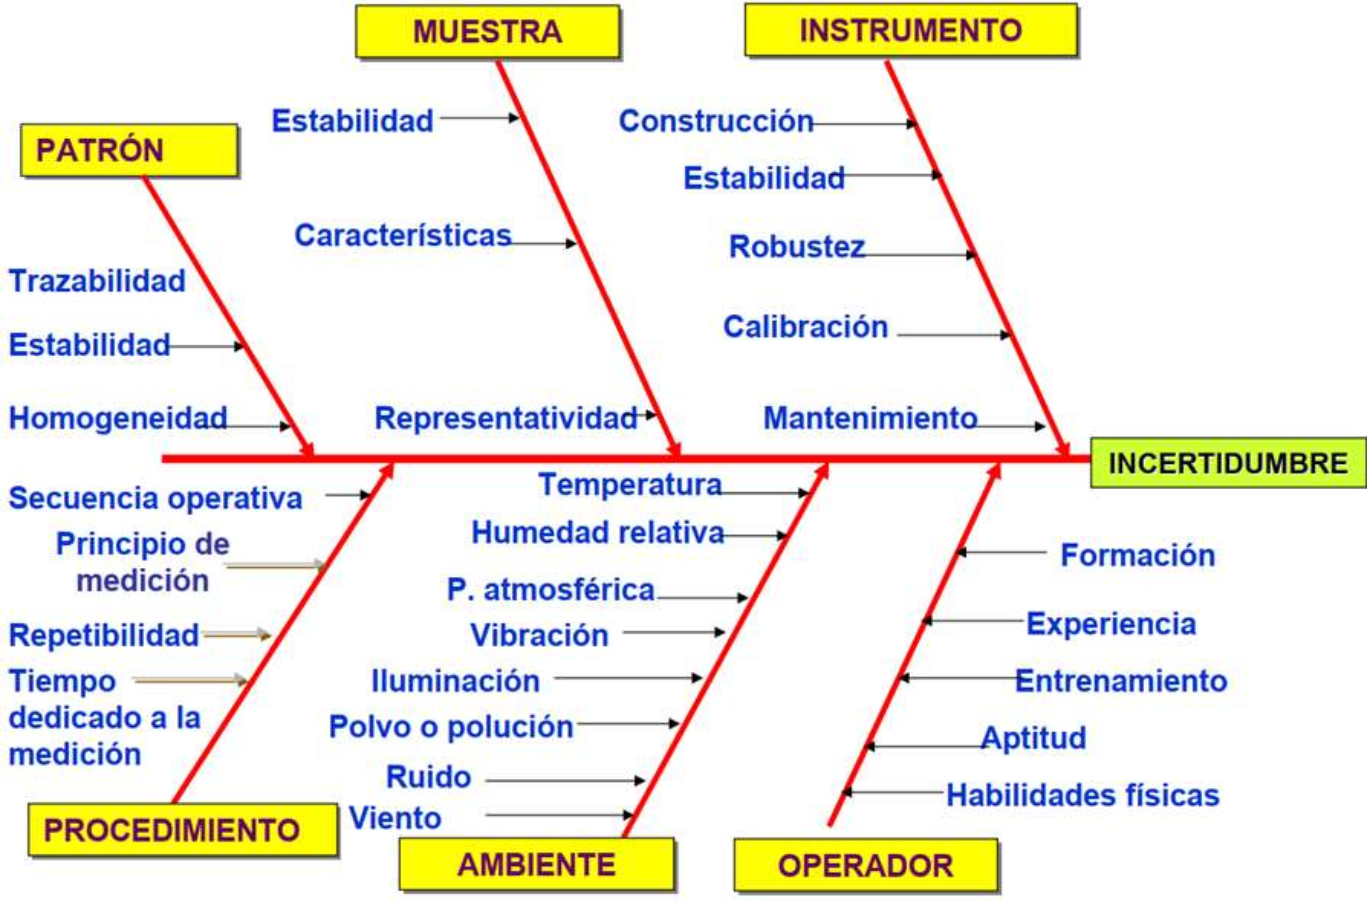
\includegraphics[width=0.8\linewidth]{Figuras/calculoIncertidumbre/diagramaPescado.png}
    \caption{Diagrama de las fuentes que producen incertidumbre en la medición de un mensurando. \cite{instrumentosMedicionesFiuba}}
    \label{fig:diagramaPescado}
\end{figure}

Existen dos tipos principales de incertidumbre: la incertidumbre de tipo A y la incertidumbre de tipo B. La incertidumbre de tipo A se evalúa mediante métodos estadísticos y se basa en datos experimentales. A partir de una serie de observaciones de una cantidad $X_{i}$, se obtiene el promedio (ecuación \ref{eq:promedioDeObservaciones}), el desvío estándar (ecuación \ref{eq:desvioEstandarDeObservaciones}) y la incertidumbre estándar (ecuación \ref{eq:incertidumbreEstandarDeObservaciones}).


\begin{equation}
    \centering
    \bar{x} = \frac{1}{n}\sum_{i=1}^{n} x_{i}
    \label{eq:promedioDeObservaciones}
\end{equation}

\begin{equation}
    \centering
    \sigma = \sqrt{\frac{1}{n-1} \sum_{i=1}^{n} (x_i - \bar{x})^2}
    \label{eq:desvioEstandarDeObservaciones}
\end{equation}

\begin{equation}
    \centering
    u(\bar{x}) = \frac{\sigma}{\sqrt{n}}
    \label{eq:incertidumbreEstandarDeObservaciones}
\end{equation}

La incertidumbre de tipo B se basa en conocimientos previos y no en datos experimentales directos. Esta puede derivarse de información contenida en manuales, certificados de calibración o la experiencia previa con el instrumento de medición. Normalmente, se especifica un entorno $\Delta = \frac{B-A}{2}$ definido como su incertidumbre expandida. Luego, para obtener la incertidumbre estándar, se divide por un número que depende de la función de distribución asumida. Para una distribución rectangular (la más usual), se divide por $\sqrt{3}$; para una distribución triangular, se divide por $\sqrt{6}$; y para una distribución de media cuadrática (RMS), donde las fuentes de incertidumbre son idénticas y aditivamente independientes, se divide por $\sqrt{2}$.

La combinación de las incertidumbres de tipo A y tipo B da lugar a la incertidumbre combinada, que proporciona una medida más completa de la incertidumbre total asociada a una medición. Generalmente, se elabora un presupuesto de incertidumbre (\textit{uncertainty budget}) a partir de todas las fuentes identificadas, con el fin de obtener una visión detallada y precisa.

Para realizar este calculo, a partir de un modelo $y = f(x_{1},x_{2}, ..., x_{n})$ que se utiliza para estimar el valor del mensurando de salida $y$, a partir de los valores de entrada $x_{1},x_{2}, ..., x_{n}$ se obtiene la incertidumbre combinada a partir de la ley de propagación de incertidumbre definida en la ecuación \ref{eq:incertidumbreCombinadaMatematica}
\begin{equation}
    \centering
    u_{c}(y) = \sqrt{\sum_{i=1}^{n} \left( \frac{\partial f}{\partial x_{i}} \right)^2 u^2(x_i)}
    \label{eq:incertidumbreCombinadaMatematica}
\end{equation}
donde la derivada parcial $\frac{\partial f}{\partial x_{i}}$ se define como el coeficiente de sensibilidad $c_{i}$ que se calcula analíticamente o en algunos casos, se puede evaluar experimental o numéricamente.

La incertidumbre combinada, definida en la ecuación \ref{eq:incertidumbreCombinadaMatematica}, puede ser ampliada mediante un factor de cobertura $k$. Este factor se obtiene calculando el valor crítico $t$ utilizando la distribución t de Student y los grados de libertad efectivos para un nivel de confianza determinado, que generalmente se encuentra entre el 68\% y el 99\%. Los grados de libertad efectivo definido en la ecuación \ref{eq:gradosDelibertadEfectivos}, representan el número de valores en un cálculo estadístico que son libres de variar. Los grados de libertad para una fuente de incertidumbre de tipo A se calcula como  $v_{i}= n_{i}-1$, donde $n_{i}$ es el numero de mediciones tomadas para cada fuente $i$. Para una fuente de incertidumbre de tipo B es mas complicado obtener los grados de libertad, pero considerando una distribución rectangular podemos asumir $v_{i} \rightarrow \infty$ \cite{Workshop_WMO2021}


\begin{equation}
    \centering
    V_{ef} = \frac{u_c^4}{\sum_{i=1}^{n} \frac{u_i^4}{v_i}}
    \label{eq:gradosDelibertadEfectivos}
\end{equation}


Esta ampliación de la incertidumbre combinada se conoce como incertidumbre expandida, la cual se muestra en la ecuación \ref{eq:incertidumbreExpandida}, proporcionando un intervalo alrededor del resultado de la medición con una alta probabilidad de contener el valor verdadero del mensurando.

% \begin{equation}
%     \centering
%     u_c = \sqrt{\sum_{i=1}^{n} (c_i \cdot u_i)^2}
%     \label{eq:incertidumbreCombinadaGral}
% \end{equation}

\begin{equation}
    \centering
    U = k \cdot u_{c}(y)
    \label{eq:incertidumbreExpandida}
\end{equation}

%%%%%%%%%%%%%%%%%%%%%%%%%%%%%%%%%%%%%%%%%%%%%%%%%%%%%%%%%%%%%%%%%%%%%%%%%%%%%%%%%%%%%%%%%%%%%%%%%%%%%%%%%%%%%%%%%%%%%%%%
%%%%%%%%%%%%%%%%%%%%%%%%%%%%%%%%%%%%%%%%%%%%%%%%%%%%%%%%%%%%%%%%%%%%%%%%%%%%%%%%%%%%%%%%%%%%%%%%%%%%%%%%%%%%%%%%%%%%%%%%
\section{Calibración y trazabilidad}\label{sec:trazabilidad}

La calibración es una operación que, bajo condiciones especificadas, establece en una primera etapa una relación entre los valores y sus incertidumbres de medida asociadas obtenidas a partir de los patrones de medida, y las correspondientes indicaciones con sus incertidumbres asociadas. En una segunda etapa, se utiliza esta información para establecer una relación que permita obtener un resultado de medida a partir de una indicación. Es importante no confundir la calibración con el ajuste del instrumento. La diferencia radica en que la calibración se obtiene a partir de comparar el Instrumento Bajo Calibración (IBC) contra un patrón de referencia estándar, bajo condiciones específicas, pero no implica modificar el instrumento. En cambio, el ajuste del instrumento implica la modificación de sus componentes pasivos o activos, de forma mecánica, eléctrica o mediante software, para que las mediciones sean lo más precisas posible, dentro de los límites de tolerancia preestablecidos por el fabricante o la aplicación del instrumento.

Para expresar la calibración, se emiten certificados de calibración en los cuales, en los puntos donde fue calibrado, se informa una función o tabla de corrección que se deriva de la diferencia entre las lecturas del patrón y las del IBC. Otro aspecto crucial que debe informarse en el certificado es la incertidumbre expandida de la corrección, la cual resulta del presupuesto de incertidumbre. El ajuste establece aplicar esta corrección a las lecturas del instrumento, lo que contribuye a mejorar la exactitud de las mediciones. 

Un certificado de calibración debe incluir la siguiente información:

\begin{itemize}
    \item \textbf{Identificación del instrumento calibrado:} Marca, modelo y número de serie del instrumento.
    \item \textbf{Identificación del patrón de referencia:} Marca, modelo y número de serie del patrón con el que se realizó la calibración.
    \item \textbf{Fecha de calibración:} Fecha en la que se realizó la calibración.
    \item \textbf{Condiciones ambientales:} Temperatura, humedad y presión atmosférica durante la calibración.
    \item \textbf{Resultados de la calibración:} Valores medidos, incertidumbres asociadas y cualquier desviación observada.
    \item \textbf{Curvas de calibración:} Gráficos de las curvas de calibración ascendente y descendente, si se incluyen.
    \item \textbf{Tablas de calibración:} Tablas con los datos de calibración, si se proporcionan.
    \item \textbf{Método de calibración:} Descripción del procedimiento utilizado para la calibración.
    \item \textbf{Certificación del laboratorio:} Información sobre la acreditación del laboratorio que realizó la calibración.
    \item \textbf{Firma y sello:} Firma del técnico responsable y sello del laboratorio.
    \item \textbf{Etiqueta:} Además se debe agregar un etiqueta en el instrumento donde se especifica la proxima fecha de calibración.
\end{itemize}

El instrumento patrón estándar también cuenta con estos parámetros en su propio certificado de calibración y son necesarios para completar el presupuesto de incertidumbre de la medición del instrumento bajo calibración (IBC), asegurando que todas las posibles fuentes de incertidumbre sean consideradas y cuantificadas.

La calibración es esencial para mantener la fiabilidad y trazabilidad a los estándares primarios. En la Figura \ref{fig:trazabilidadMetrologica} se muestra cómo, a partir de un patrón internacional, se calibra un patrón nacional tomando como referencia la incertidumbre del patrón internacional. De esta forma, en sentido descendente, se tienen incertidumbres cada vez mayores hasta llegar al equipo de medición. Por otro lado, en sentido inverso, la trazabilidad es una propiedad de un resultado de medida por la cual dicho resultado puede relacionarse con un valor de referencia, nacional o internacional, a través de una cadena ininterrumpida y documentada de calibraciones, donde cada una contribuye a la incertidumbre de la medición.

\begin{figure}[H]
    \centering
    \includegraphics[width=0.7\linewidth]{Figuras/calculoIncertidumbre/trazabilidadMetrologica.png}
    \caption{Trazabilidad metrológica. \cite{instrumentosMedicionesFiuba}}
    \label{fig:trazabilidadMetrologica}
\end{figure}

%%%%%%%%%%%%%%%%%%%%%%%%%%%%%%%%%%%%%%%%%%%%%%%%%%%%%%%%%%%%%%%%%%%%%%%%%%%%%%%%%%%%%%%%%%%%%%%%%%%%%%%%%%%%%%%%%%%%%%%%

\section{Modelo teórico de medición}\label{sec:modelo_teoricos}

El modelo de medición utilizado para calcular la incertidumbre de los anemómetros se muestra en la ecuación \ref{eq:ModeloIncertidumbre}. Este modelo se basa en una comparación, donde se obtiene la corrección del mensurando bajo calibración a partir de la diferencia de medición en un punto determinado y bajo condiciones ambientales controladas, entre un patrón calibrado y el instrumento bajo calibración.

\begin{equation}
    CV_{IBC} = \overbrace{V_{p} + CV_{p}}^{V_{ref}} - V_{IBC}
    \label{eq:ModeloIncertidumbre}
\end{equation}
donde se define:

\begin{itemize}
    \item $V_{IBC}$ representa el valor de viento medido con el anemómetro bajo calibración.
    \item $CV_{IBC}$ representa la corrección del anemómetro bajo calibración.
    \item $V_{p}$ representa el valor de viento medido con el anemómetro patrón.
    \item $CV_{p}$ representa la corrección de viento del anemómetro patrón, obtenida a partir de su certificado de calibración.
\end{itemize}

A partir de la ecuación \ref{eq:ModeloIncertidumbre} y tomando en cuenta las fuentes de incertidumbre, definidas en la tabla \ref{tab:fuenteIncert} se realiza el cálculo de la incertidumbre combinada de la corrección, como la suma de los cuadrados de las incertidumbres estándar de cada fuente, como se muestra en la ecuación \ref{eq:incertidumbreCombinada}.

\begin{equation}
    u^{2}(CV_{IBC}) = u^{2}(V_{ref})+u^{2}(V_{IBC})+u^{2}(\text{túnel de Viento})
    \label{eq:incertidumbreCombinada}
\end{equation}
donde se define:

\begin{itemize}
    \item $u^{2}(CV_{IBC})$ es la incertidumbre estándar de la corrección del anemómetro bajo calibración.
    \item $u^{2}(V_{ref})$ representa la suma de todas las fuentes de incertidumbre estándar debidas al patrón de referencia.
    \item $u^{2}(V_{IBC})$ representa la suma de todas las fuentes de incertidumbre estándar debidas al anemómetro bajo calibración.
    \item $u^{2}(\text{túnel de Viento})$ es la contribución de incertidumbre estándar referida al túnel de viento, quien se encarga de generar condiciones de velocidad y dirección de viento.
\end{itemize}
%%%%%%%%%%%%%%%%%%%%%%%%%%%%%%%%%%%%%%%%%%%%%%%%%%%%%%%%%%%%%%%%%%%%%%%%%%%%%%%%%%%%%%%%%%%%%%%%%%%%%%%%%%%%%%%%%%%%%%%%
\section{Fuentes de incertidumbre}\label{sec:fuentesDeIncertidumbre}
\newcommand{\descCalibracion}{Incertidumbre expandida especificada  en el certificado de calibración.}
\newcommand{\descAjusteCalibracion}{Desvío estándar del ajuste lineal con los datos discretos del certificado de calibración.}
\newcommand{\descResolucionInstrumento}{Mínima diferencia entre valores indicados por el instrumento bajo calibración a través de su sistema de adquisición o lectura de datos.}
\newcommand{\descResolucionPatron}{Solo se debe agregar en caso de utilizar un sistema de lectura o adquisición distinto al que fue calibrado.}
\newcommand{\descRepetibilidad}{Desvío estándar de la media aritmética de las mediciones.}
\newcommand{\descHisteresis}{Diferencia entre los valores de mediciones realizadas en los ciclos ascendente y descendente.}
\newcommand{\descFactorBloqueo}{Incertidumbre asociada al factor de bloqueo que se define como la relación entre el área transversal del túnel de viento y el área efectiva del anemómetro, proyectada en el plano transversal.}
\newcommand{\descHomogeneidad}{Variación espacial del flujo de aire dentro del túnel.}
\newcommand{\descAjusteHomogeneidad}{Desvío estándar del ajuste lineal con los datos discretos del certificado de homogeneidad.}
\newcommand{\descEstabilidad}{Variación temporal del flujo de aire dentro del túnel.}
\newcommand{\descAjusteEstabilidad}{Desvío estándar del ajuste lineal con los datos discretos del certificado de estabilidad.}
\newcommand{\descFactorCalib}{Incertidumbre asociada al factor de calibracion que proporciona la relación entre las condiciones en la posición de medición de referencia y las condiciones en la posición del IBC.}

\begin{table}
\centering
\fontsize{9}{8}\selectfont
\begin{tblr}{
    colspec = {Q[c,1.1cm] Q[c,1.2cm] Q[c,6cm] Q[c,0.8cm] Q[c,1.9cm] Q[c,2.1cm]},
    cells = {c}, % Centra todas las celdas por defecto
    row{1} = {Sail}, % Aplica el estilo "Sail" a la primera fila
    cell{1}{1} = {c=2}{}, % La celda en la fila 1, columna 1 se extiende a dos columnas
    cell{2}{1} = {r=6}{}, % La celda en la fila 2, columna 1 se extiende a seis filas
    cell{8}{1} = {r=5}{}, % La celda en la fila 8, columna 1 se extiende a cinco filas
    cell{13}{1} = {r=4}{}, % La celda en la fila 13, columna 1 se extiende a tres filas
    vlines, % Añade líneas verticales entre todas las columnas
    hline{1-2,8,13,17} = {-}{}, % Añade líneas horizontales completas en las filas 1-2, 8, 13 y 17
    hline{3-7,9-12,14-16} = {2-6}{}, % Añade líneas horizontales parciales en las filas 3-7, 9-12 y 14-15
}
Fuentes de Incertidumbre    &                                   & Descripción               & Tipo  & Distribución de probabilidad & Factor de normalización \\
Patrón                      & Calibración                       & \descCalibracion          & B                          &  N                           &  2                      \\
                            & Ajuste de calibración         & \descAjusteCalibracion    & A                           & N                            &  1                      \\
                            & Resolución   & \descResolucionPatron& B                           & R                            &  $\sqrt{3}$                      \\
                            & Repetibilidad                     & \descRepetibilidad        & A                           & N                            & $\sqrt{n}$, n muestras                      \\
                            & Histéresis                        & \descHisteresis           & B                          &  R                           & $\sqrt{3}$                       \\
                            & Factor de bloqueo             & \descFactorBloqueo        & B                          & RMS                             & 1                       \\
Túnel de viento             & Homogeneidad                      & \descHomogeneidad         & B                          & R                            & $\sqrt{3}$                       \\
                            & Ajuste de la homogeneidad     & \descAjusteHomogeneidad   & A                          & N                            & 1                       \\
                            & Estabilidad                       & \descEstabilidad          & B                           & R                            & $\sqrt{3}$                        \\
                            & Ajuste de la estabilidad      & \descAjusteEstabilidad    & A                          & N                            & 1                       \\
                            & Factor de calibración                          & \descFactorCalib              & B                          & RMS                            & 1\\
IBC                         & Resolución                & \descResolucionInstrumento& B                          & R                             & $\sqrt{3}$                        \\
                            & Repetibilidad                     & Lo mismo que la definición para el patrón        & A                          & N                            & $\sqrt{n}$, n muestras                        \\
                            & Histéresis                        & Lo mismo que la definición para el patrón           & B                           & R                            & $\sqrt{3}$                        \\
                            & Factor de bloqueo             & Lo mismo que la definición para el patrón        & B                          & RMS                             & 1                       \\
\end{tblr}
\caption{Fuentes de incertidumbre evaluadas para el presupuesto de incertidumbre de un anemómetro bajo calibración en el túnel de viento del SMN.}
\label{tab:fuenteIncert}
\end{table}

En particular se va a considerar las fuentes de incertidumbre debidas a:
\begin{itemize}
    \item El sensor bajo calibración.
    \item El sensor patrón de referencia.
    \item El túnel de viento.
\end{itemize}

En la tabla \ref{tab:fuenteIncert} se detallan las fuentes de incertidumbre que se evaluarán en el presupuesto de incertidumbre para cada punto de viento configurado. En la segunda columna se nombra el tipo de fuente y en la tercera columna se da una breve descripción de cada una. Luego, cada incertidumbre se clasifica según el tipo A o B, en función de cómo fue determinada. En la quinta columna se especifica el tipo de distribución probabilística. Finalmente, en la última columna se detalla el factor de normalización por el cual se debe dividir para obtener la incertidumbre estándar de cada fuente. Vale la pena destacar que la histéresis también se utiliza como indicador de la no linealidad del instrumento bajo calibración; una histéresis alta sugiere que el instrumento muestra un comportamiento diferente cuando la magnitud medida está aumentando en comparación a cuando está disminuyendo. Por otro lado, tanto el factor de bloqueo como en factor de calibración deben ser calculados previamente para luego obtener su correspondiente incertidumbre estándar.

%%%%%%%%%%%%%%%%%%%%%%%%%%%%%%%%%%%%%%%%%%%%%%%%%%%%%%%%%%%%%%%%%%%%%%%%%%%%%%%%%%%%%%%%%%%%%%%%%%%%%%%%%%%%%%%%%%%%%%%%



